%-*-latex-*-
The goal here is to compute an approximation of the value of $\pi$ using the
\lq\lq Monte--Carlo" method. The Monte--Carlo method is a very famous
approximation method for computing numbers and has many important applications
in simulation, engineering sciences, game theory, etc. The idea is very simple.
Look at the following:
\begin{center}
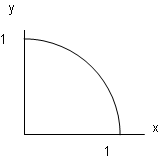
\includegraphics[scale=0.5]{pic1.png}
\end{center}
This is the quarter circle of radius $1$. The area of a full circle of radius
$r$ is $\pi r^2$. For the circle of radius $1$, the area would be $\pi 1^2$
which is $\pi$. So our quarter circle would have an area of $\pi / 4$. (Here,
the $/$ refers to mathematical division and not integer division.)

Suppose we generate a lot of random points in the square with corners
$(0,0), (0,1), (1,0), (1,1)$:
\begin{center}
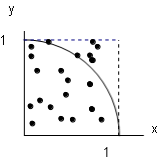
\includegraphics[scale=0.5]{pic2.png}
\end{center}

and consider the total number of random points and the number of points that
hit the interior of the quarter circle. Then clearly
\[
\frac{\text{Number of points in quarter circle}}
{\text{Total number of points}} 
\approx
\frac{\text{Area of quarter circle}}
{\text{Area of square}}
\]
($\approx$ means \lq\lq approximately".) But this is just
\[
\frac{\text{Number of points in quarter circle}}
{\text{Total number of points}}
\approx
\frac{\pi / 4}{1}
\]
which gives
\[
\pi
\approx
\frac{4 * \text{(Number of points in quarter circle)}}
{\text{Total number of points}}
\]

[ASIDE: In general, the Monte--Carlo method can be used to approximate areas.
This is not the only method used to approximate values. In fact, the
Monte--Carlo method is usually very slow in the sense that you need to
generate many random events -- which in this case is the generation of random
points in the square -- before you get a good approximation. Using the power
series method one can get an extremely good approximation of $\pi$ with only
$100$ iterations.]

Complete the following skeleton code. You should not add any code to
\verb!main()!.  

\begin{Verbatim}[frame=single]
//------------------------------------------------------------------------
// Prompts and returns the number of points entered by the user
//------------------------------------------------------------------------
int getNumPoints()
{
}


//------------------------------------------------------------------------
// randunit() returns a random double from 0.0 to 1.0
//------------------------------------------------------------------------
double randunit()
{
}


//------------------------------------------------------------------------
// pointIsInCircle(x, y) returns true if the point (x,y) is in the quarter
// circle
//------------------------------------------------------------------------
bool pointIsInCircle(double x, double y)
{
}


//------------------------------------------------------------------------
// printRunningApproximation(i, inCircle) prints for instance:
//
// 1000000         785219          3.1408760000
//
// (See Test 1)
// if i is 1000000 and inCircle is 78219. The third column is the 
// approximation of pi with the number of points generated at this point 
// (i.e., i) and the number of points in the quarter circle (i.e. 
// inCircle)
//------------------------------------------------------------------------
void printRunningApproximation(int i, int inCircle)
{
}


//------------------------------------------------------------------------
// printSummary(n, inCircle) prints for instance:
//
// The Pi-minator strikes again ...
// Final approximation of pi: 3.1415482200
// Number of points generated: 1000000000
//
// (See Test 1) if n is 1000000000 and inCircle is 785387055.
//------------------------------------------------------------------------
void printSummary(int n, int inCircle)
{
}


int main()
{
    srand((unsigned int) 0);
    std::cout << std::fixed << std::setprecision(10);

    int n = getNumPoints();

    int inCircle = 0;  // Counts the number of random points in 
                       // the quarter circle
    for (int i = 1; i <= n; ++i)
    {
        // Generate random point (x,y) in the square
        double x = randunit();
        double y = randunit();

        // Increment inCircle if (x,y) is in the quarter circle
        if (pointIsInCircle(x, y))
        {
            ++inCircle;
        }

        printRunningApproximation(i, inCircle);
    }

    printSummary(n, inCircle);

    return 0;
}
\end{Verbatim}

Refer to \textbf{Test 1} for the output. Some of the output is not shown since
the output is very long. Note that the first two columns have width of $16$.
The numbers in the third column have $10$ decimal places after the decimal
point. Furthermore, note that the running approximation is printed only after
every $1000000$ points are generated. Note also that the \verb!rand()!
function in your compiler might work differently from mine. However, the
approximations should still move toward the value of $\pi$.


\resett
\nextt
(Only part of the output is shown.)
\begin{console}[frame=single, commandchars=\\\{\}]
Number of points to generate: \userinput{1000000000}
1000000         785219          3.1408760000
2000000         1571143         3.1422860000
3000000         2356627         3.1421693333
4000000         3141318         3.1413180000
\emph{... output not shown ...}
998000000       785230080       3.1415486297
999000000       785308538       3.1415483068
1000000000      785387055       3.1415482200
The Pi-minator strikes again ...
Final approximation of pi: 3.1415482200
Number of points generated: 1000000000
\end{console}
